\section{Machine Learning Models}

\begin{frame}{Tree-Based Models: RF \& XGBoost}
    \textbf{Random Forest (Baseline - Bagging):}
    \begin{itemize}
        \item Minimizes \textit{Gini Impurity}: $ G = 1 - \sum p_i^2 $
        \item Robust against overfitting, excellent interpretability.
    \end{itemize}
    \vspace{0.2cm}
    \textbf{XGBoost (Boosting):}
    \begin{itemize}
        \item Builds sequential trees correcting residual errors.
        \item Optimizes Log-Loss + Regularization ($\Omega$): $\mathcal{L}^{(t)} = \sum l(y_i, \hat{y}_i) + \Omega(f_t)$
    \end{itemize}
    \vspace{0.2cm}
    \textbf{Hyperparameter Optimization:}
    \begin{itemize}
        \item \texttt{RandomizedSearchCV} with 3-fold CV. Metric optimized: \textbf{ROC AUC}.
    \end{itemize}
\end{frame}

\begin{frame}{Feature Importance Analysis}
    \begin{columns}
        \begin{column}{0.45\textwidth}
            \textbf{Key Insights (Random Forest):}
            \begin{itemize}
                \item \texttt{action\_type} dictates outcome more than spatial position ($\sim$40\% weight).
                \item Validates the extensive feature engineering phase.
            \end{itemize}
        \end{column}
        \begin{column}{0.55\textwidth}
            \begin{figure}
                \centering
                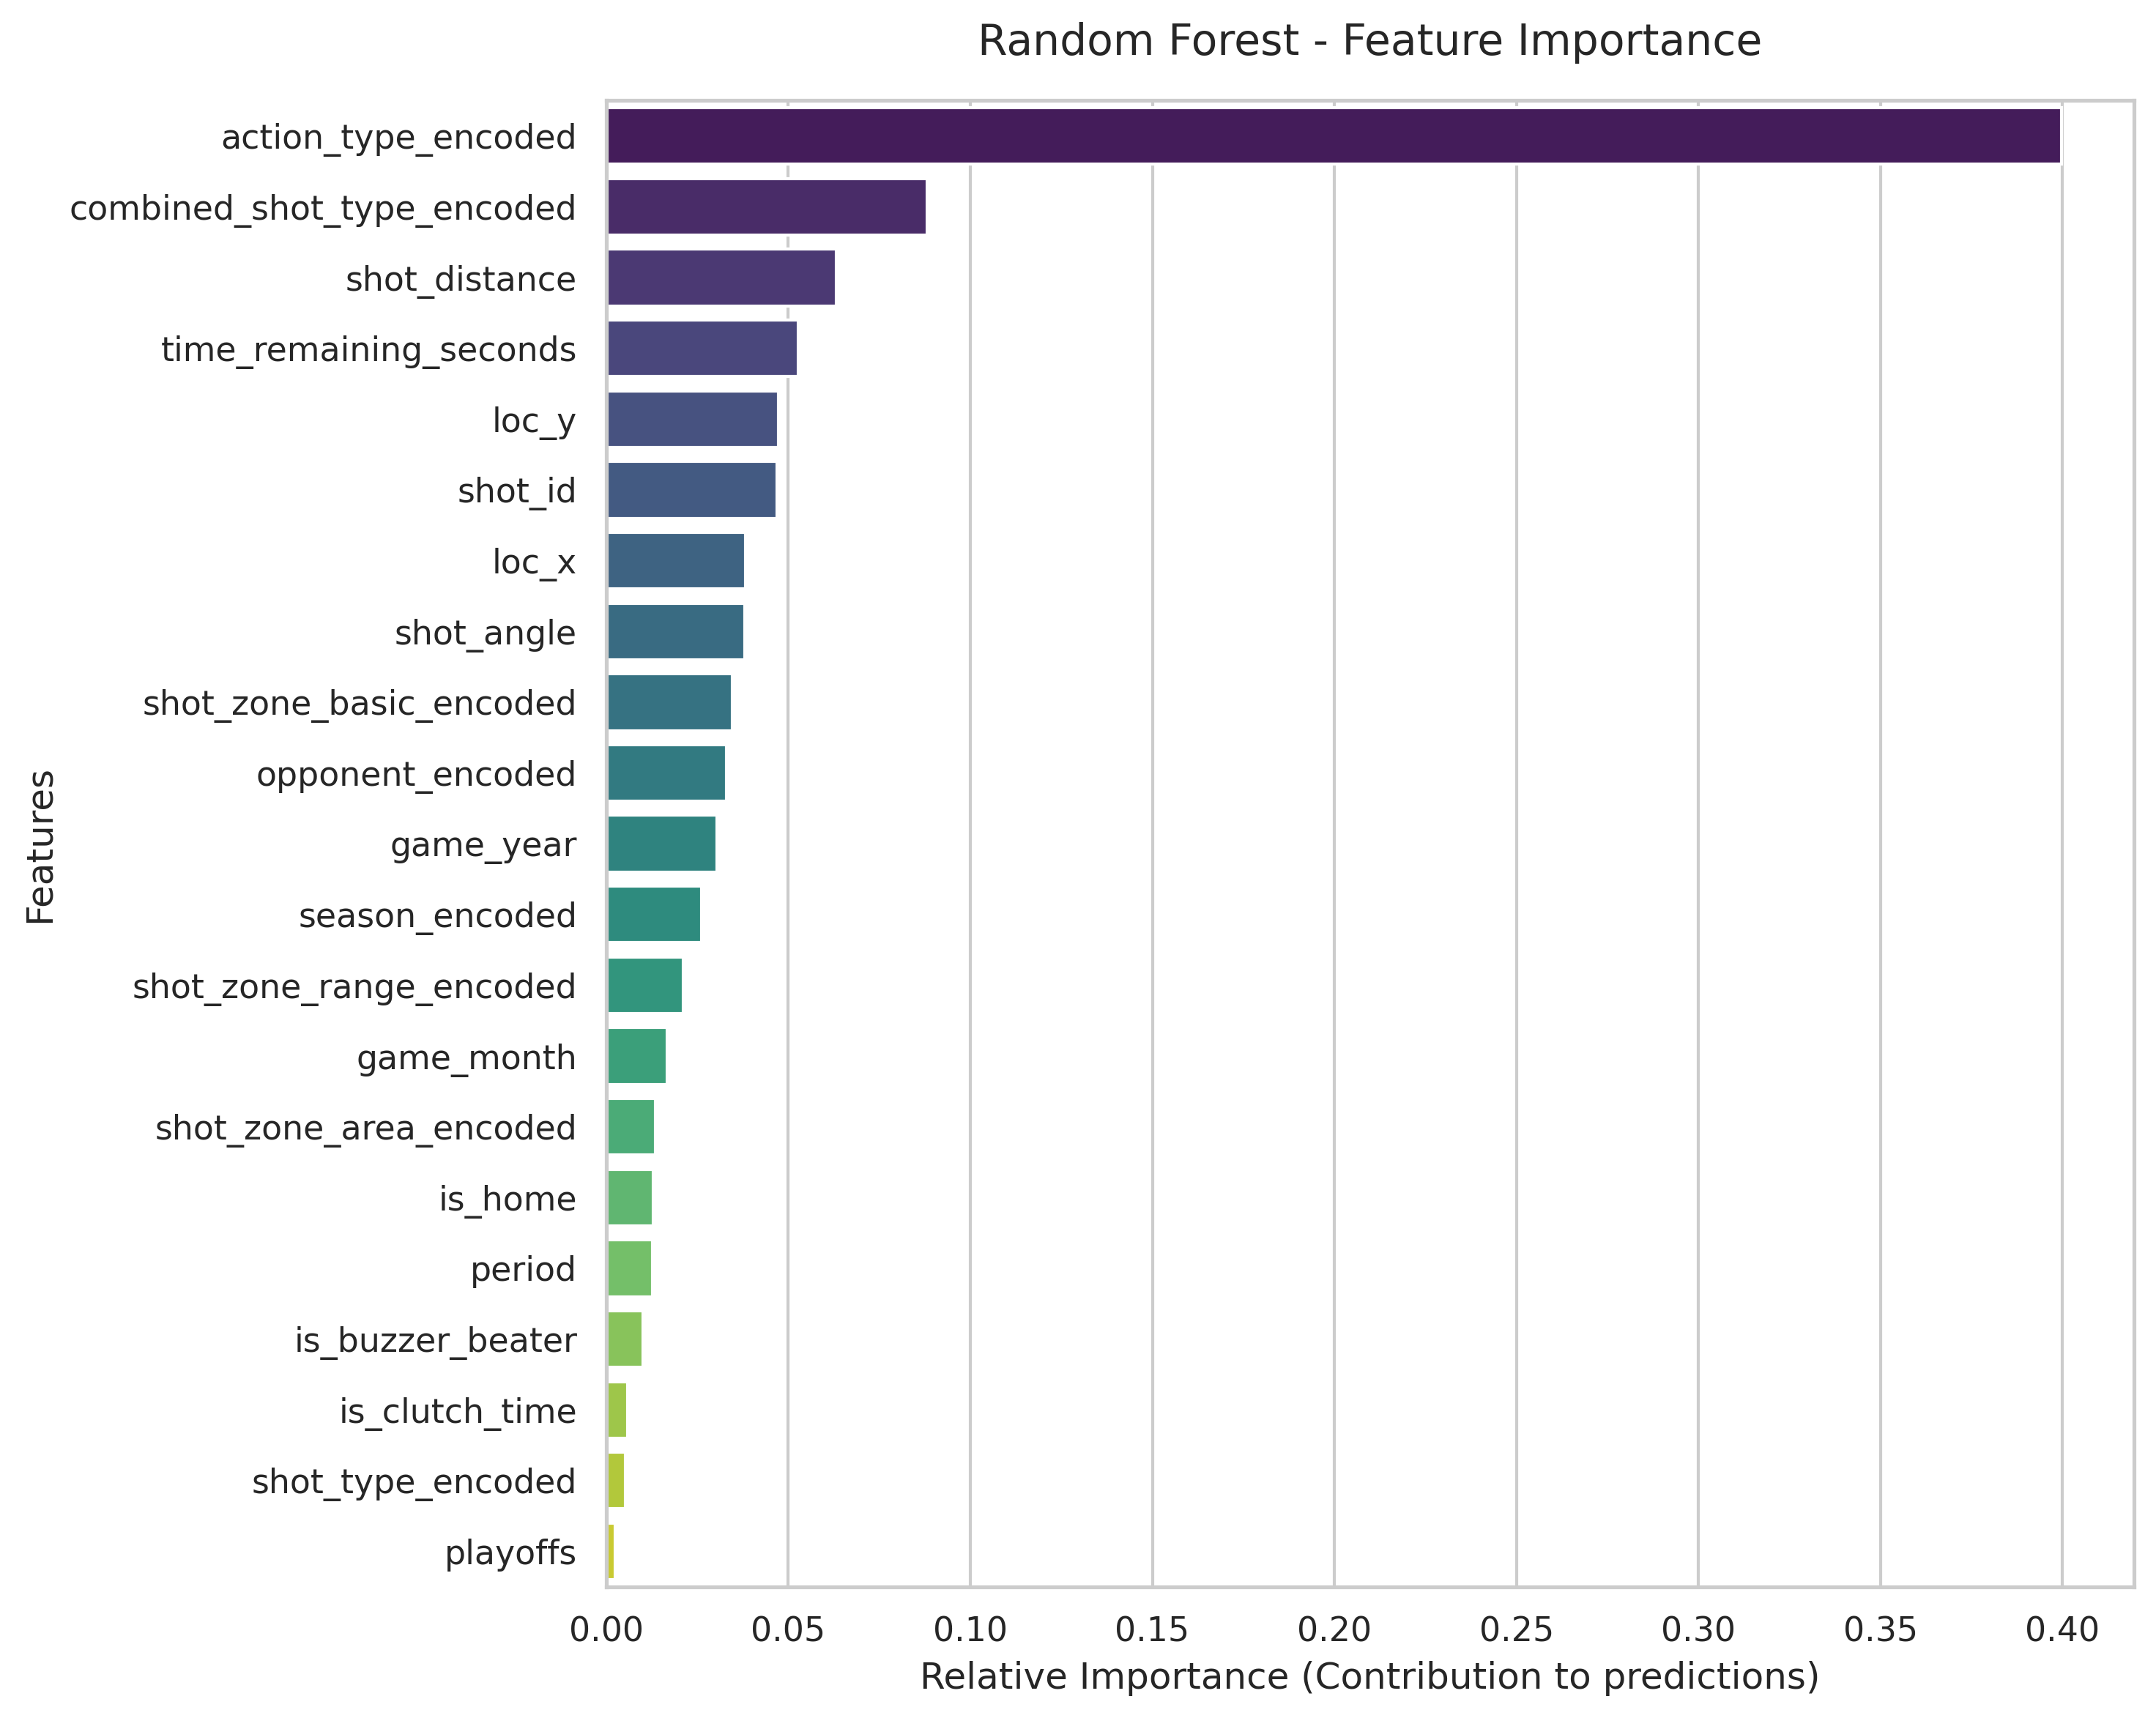
\includegraphics[width=\textwidth]{img/feature_importance.png}
            \end{figure}
        \end{column}
    \end{columns}
\end{frame}